% Provenance (never printed): see sources/outline_sources.md (Year 2: climate archives and proxies;
% foraminiferal and ice isotopes; Mg/Ca; pollen; speleothems; tree rings; dating the archives).
% Calibrations after Miller et al. (2020), Groeneveld et al. (2019) and Morley et al. (2024); ice
% cores after White (Geochemistry, ch. 9), Werner et al. (2018) and the EPICA Dome C file of Jouzel
% et al. (2007); age model after Svensson et al. (2008); deep-water context after Wharton et al.
% (2026); figures from figdata/bachelor-2/proxies.py (data/derived lr04, edc-temperature,
% co2-icecore); values of the exercises and problem computed in the Book 4 scratch calculator
% calc/ch24.py.
\chapter{气候档案与代用指标}\label{ch:b2:climate-proxies}

1955 年，一位年轻的地球化学家在一篇论文中报告了微小有孔虫壳体的氧同位素，这些壳体取自
海底岩心，并在其中发现过去 \num{600000} 年间的 15 个冰期–间冰期旋回。
他主要把它们读作温度的记录，只把约五分之一的
变化归因于陆地上储存的冰。十八年后，沙克尔顿和奥普代克得出了相反的结论：
主要效应是同位素较轻的水储存于冰盖之中。
同样的壳体，同样的数字，两种解读。方解石壳体记录了其形成时所处水体的
温度与成分，而海水的成分
取决于陆地上有多少冰。本章讨论这类记录、保存记录的档案、
由其中读取的代用指标、它们如何借助温度计标定，
如何定年，以及如何分辨同一壳体所携带的两种信号。
% ledger: white13c9:paleo-history

\begin{recall}
\textbf{来自中学各分册}：\omterm{def:b2:climate-proxies:proxy}{气候档案}和代用指标、冰芯、冰期和间冰期、
末次盛冰期（约 \num{23000} 至 \num{19000} 年前）、孢粉
分析。\textbf{来自本科一年级分册}：放射性测年、放射性碳年龄及其
标准曲线；钙质软泥，由颗石和有孔虫壳体组成。
\textbf{来自\cref{ch:b2:isotope-geochemistry}}：\omterm{def:b2:isotope-geochemistry:standards}{同位素参考标准} \omterm{def:b2:isotope-geochemistry:standards}{VSMOW} 和 \omterm{def:b2:isotope-geochemistry:standards}{VPDB}
（\cref{def:b2:isotope-geochemistry:standards}）以及\omterm{prop:b2:isotope-geochemistry:mwl}{大气降水线}，$\delta\mathrm{D}
\approx 8\,\delta^{18}\mathrm{O} + 10$（\cref{prop:b2:isotope-geochemistry:mwl}）。\textbf{来自
化学各分册}：$\delta$ 值和分馏系数。\textbf{来自
数学各分册}：最小二乘直线。
\end{recall}
% ledger: ipcc:lgm-cooling, kc98:mwl, kc98:standards

\section{档案与代用指标}\label{sec:b2:climate-proxies:archives}

更早的气候信息都读取自各种材料，仪器观测气候的历史很短。
这些材料在气候作用下逐层生长或沉积：雪在
极地冰盖上化为冰，壳体落到海底，树木年轮、珊瑚、洞穴的
沉积物与湖泊的淤泥。中学各分册称它们为档案，称其中测得的量为
代用指标；现在需要更精确的术语。

\begin{definition}[气候档案；气候代用指标]\label{def:b2:climate-proxies:proxy}
称\emph{气候档案}\index{气候档案}为一种天然材料，它
逐层或逐环渐进地积累，并保存了各部分形成时所处环境的物理、化学或生物
特征。称\emph{气候代用指标}\index{气候代用指标}为在档案中测得的一个量，它依赖于某个气候变量，
如温度、降水量或冰的体积，
通过一种可以标定的关系，
因而可代替一个从未做过的该变量测量。
\end{definition}
% ledger: ncei:proxy, ncei:paleocean

决定档案能说明什么的有三个性质：分辨率（一个样品所覆盖的时间跨度）、
追溯范围（能回溯到多久以前）以及定年方式。具有年层的档案可以逐年读取，
并通过计数定年；其他档案则需要放射性年龄，或与一个已定年的记录对比。
下表比较了本章的各类档案。

\begin{center}
\small
\begin{tabular}{>{\raggedright\arraybackslash}p{0.17\linewidth}>{\raggedright\arraybackslash}p{0.27\linewidth}>{\raggedright\arraybackslash}p{0.21\linewidth}>{\raggedright\arraybackslash}p{0.24\linewidth}}
\hline
档案 & 本章的代用指标 & 年层 & 定年方式 \\
\hline
深海沉积物 & 有孔虫的 $\delta^{18}$O 和 Mg/Ca & 无 & 放射性碳，与
已定年记录对比 \\
极地冰 & 冰的 $\delta$D 和 $\delta^{18}$O，气泡中的空气 & 厚冰芯的
上部 & 计数层位，已定年的火山层 \\
树木年轮 & 年轮宽度、木材密度、同位素 & 有 & 计数并\omterm{def:b2:climate-proxies:dendro}{交叉定年}年轮 \\
\omterm{def:b2:climate-proxies:archives}{洞穴沉积物} & $\delta^{18}$O & 部分有 & 放射性测年 \\
湖泊沉积物 & \omterm{def:b2:climate-proxies:archives}{纹泥}、孢粉 & 在有\omterm{def:b2:climate-proxies:archives}{纹泥}处 & 计数\omterm{def:b2:climate-proxies:archives}{纹泥} \\
\hline
\end{tabular}
\end{center}
% ledger: ncei:proxy, ncei:paleocean, ncei:tree-ring, ncei:speleothem, mccarthy23:varves, svensson08:gicc05, noaa:gisp2-layers, bebchuk26:crossdating

代用指标从来不是单一变量的纯测量。树木年轮的宽度既取决于夏季的温暖程度，
也取决于降雨；壳体的 $\delta^{18}$O 取决于水温，
也取决于水的同位素组成。古气候学家的工作在于找到一种代用指标，其对所求变量的依赖
关系要强且已知，独立测定其他影响，并
为样品定年。

\section{碳酸盐壳体中的氧同位素}\label{sec:b2:climate-proxies:oxygen}

有孔虫是单细胞原生生物，其中许多种类分泌方解石壳体；浮游
物种漂浮于表层海水中，底栖物种则生活在海底沉积物之上或其中。
它们的壳体堆积成本科一年级分册中所说的钙质软泥，而
方解石的 $\delta^{18}$O 可在岩心每厘米取出的
少量壳体上测得。
% ledger: ucmp:forams, ncei:paleocean

\begin{history}[同一记录的两种解读]
尤雷于 1947 年计算了氧在方解石与水之间的分馏如何依赖于
温度，并提出碳酸盐可以记录其形成时的温度。切萨雷·埃米利亚尼
当时是他的学生，测量了取自世界各大洋活塞岩心的有孔虫 $\delta^{18}$O，
并于 1955 年发表记录，其中含 15 个冰期–间冰期旋回，覆盖
\num{600000} 年，并把约 \qty{20}{\percent} 的变化归因于冰量。
1973 年，沙克尔顿和奥普代克得出结论：同位素较轻的水
储存于冰盖中是主要效应。生命效应，即物种偏离平衡的偏差，
以及埋藏后氧与孔隙水的交换，对最近几百万年的
壳体通常并不很重要；起决定作用的是水的同位素组成。
\end{history}
% ledger: white13c9:paleo-history

\subsection*{温度}

与水处于平衡时生长的方解石比水更富含 \textsuperscript{18}O，
水温越低，富集程度越大，这正是尤雷的计算所示。
若干经验标定把
温度与方解石的 $\delta^{18}$O（\omterm{def:b2:isotope-geochemistry:standards}{VPDB} 标度）
与水的（\omterm{def:b2:isotope-geochemistry:standards}{VSMOW} 标度）之差相联系。对深海，底栖
壳体通常采用一种简化形式。

\begin{proposition}[底栖生物校准]\label{prop:b2:climate-proxies:benthic}
对于深海温度（低于约 \qty{13}{\celsius}）下的底栖有孔虫，
\[
  T = 16.1 - 4.76\,\bigl[\delta^{18}\mathrm{O}_{\mathrm{b}} - (\delta^{18}\mathrm{O}_{\mathrm{sw}} -
  0.27)\bigr],
\]
其中 $T$ 的单位为 \unit{\celsius}，$\delta^{18}\mathrm{O}_{\mathrm{b}}$ 为贝壳的值（千分值，
\omterm{def:b2:isotope-geochemistry:standards}{VPDB}），$\delta^{18}\mathrm{O}_{\mathrm{sw}}$ 为海水的值（千分值，\omterm{def:b2:isotope-geochemistry:standards}{VSMOW}）；
0.27 这一项把水的标度换算为方解石的标度。海水成分不变时，降温 \qty{1}{\celsius}
使 $\delta^{18}\mathrm{O}_{\mathrm{b}}$ 升高 $1/4.76 = 0.21$ 千分值。
\end{proposition}
\admitted
% ledger: miller20:paleotemp, groeneveld19:anand

简化前的完整方程含一个较小的二次项，
$T = 16.1 - 4.64x + 0.09x^2$，式中 $x$ 为两个 $\delta$ 值之差；浮游有孔虫贝壳
各有其校准式，形式相同，例如 $T = 14.9 - 4.8\,[\delta^{18}\mathrm{O} -
(\delta^{18}\mathrm{O}_{\mathrm{sw}} - 0.27)]$。它们共同存在一个难点：贝壳只给出一个
数值 $\delta^{18}\mathrm{O}_{\mathrm{b}}$，而方程含两个未知量 $T$ 与
$\delta^{18}\mathrm{O}_{\mathrm{sw}}$。需引入第二个独立的代用指标，才能将二者分开。
% ledger: miller20:paleotemp, groeneveld19:anand

\subsection*{冰量效应}

从海面蒸发的水所含 \textsuperscript{18}O 少于海水；蒸气
向极地输送并降雨或降雪后，其 \textsuperscript{18}O 进一步减少，构成
冰盖的雪是地球上最轻的水之一：格陵兰冰的 $\delta^{18}$O 为 $-30$ 至 $-35$
千分值，南极冰低至 $-50$。冰盖增长时，轻同位素锁存于陆地，
留下的海洋则变得更重。
% ledger: nasaeo:o18, white:d18o

\begin{definition}[冰量效应]\label{def:b2:climate-proxies:ice-volume}
称\emph{冰量效应}\index{冰量效应}为由大陆冰盖的增长或消退
引起的整个海洋氧同位素组成的变化，这些冰盖储存的水贫
\textsuperscript{18}O；其作用使海中形成的每种碳酸盐的 $\delta^{18}$O 产生相同的偏移，
与温度无关。
\end{definition}
% ledger: nasaeo:o18, white13c9:ice-volume, miller20:paleotemp

\begin{omfigure}
\centering
\begin{tikzpicture}[font=\scriptsize, >=Stealth]
\foreach \col/\title in {0/{a\enspace 现今}, 7.0/{b\enspace 冰期极盛期}} {
  \begin{scope}[shift={(\col,0)}]
  \node[anchor=south west] at (0,3.3) {\textbf{\title}};
  \fill[brown!30] (3.6,0) -- (6.4,0) -- (6.4,1.6) -- (3.6,1.2) -- cycle;
  \end{scope}
}
% today: full ocean, small ice sheet
\fill[ocBlue!25] (0,0) rectangle (3.6,1.2);
\node[align=center] at (1.75,0.55) {海洋 \\$\delta^{18}\mathrm{O} = 0$};
\fill[white, draw=black!50] (5.2,1.43) .. controls (5.6,1.95) and (6.2,1.95) .. (6.4,1.6) -- cycle;
\node at (5.0,0.65) {冰，$-40$};
\draw[black!50] (5.0,0.85) -- (5.7,1.55);
\draw[->, thick, ocBlue] (1.6,1.35) .. controls (2.4,2.9) and (4.6,2.9) .. (5.6,2.05);
\node at (3.4,3.0) {蒸气，轻};
% glacial: lower sea, big ice sheet
\begin{scope}[shift={(7.0,0)}]
\fill[ocBlue!35] (0,0) rectangle (3.6,0.85);
\draw[densely dashed] (0,1.2) -- (3.6,1.2);
\node[anchor=south west, align=left] at (0.05,1.2) {今日 \\海平面};
\draw[<->] (3.35,0.85) -- (3.35,1.2);
\node[anchor=east] at (3.3,1.02) {\qty{130}{m}};
\node[align=center] at (1.6,0.42) {海洋，$\delta^{18}\mathrm{O} = +1.46$};
\fill[white, draw=black!50] (3.6,1.2) .. controls (4.0,2.6) and (6.0,2.7) .. (6.4,1.6) -- cycle;
\node at (5.1,1.85) {冰，$-40$};
\draw[->, thick, ocBlue] (2.15,0.9) .. controls (2.3,2.6) and (3.3,3.0) .. (4.3,2.6);
\end{scope}
\end{tikzpicture}
\par\smallskip{\small \omterm{def:b2:climate-proxies:ice-volume}{冰量效应}（示意图，未按比例绘制）：为冰盖供给水分的蒸气
\textsuperscript{18}O 贫化，因此把相当于 \qty{130}{m} 海平面的水储存为
$\delta^{18}\mathrm{O} = -40$ 千分值的冰，使海洋变重 \num{1.46} 千分值
（见\cref{prop:b2:climate-proxies:mass-balance}）。数值以千分值表示，标度为 \omterm{def:b2:isotope-geochemistry:standards}{VSMOW}。}
\end{omfigure}
% ledger: nasaeo:o18, miller20:ice-cal, ipcc:lgm-sea

这一偏移有多大？质量平衡可以回答这一问题，
前提是已知冰的体积及其平均同位素组成。

\begin{proposition}[由质量平衡求冰量效应]\label{prop:b2:climate-proxies:mass-balance}
设现今海洋的平均深度为 $H$，其 $\delta^{18}$O 为 0（\omterm{def:b2:isotope-geochemistry:standards}{VSMOW}）。若移去一层
厚度为 $h$ 的海水，并以平均组成为
$\delta_{\mathrm{ice}}$ 的冰储存于陆地，海洋面积保持不变，剩余海洋具有
\[
  \Delta\delta^{18}\mathrm{O}_{\mathrm{sw}} = \frac{-h\,\delta_{\mathrm{ice}}}{H - h}.
\]
当 $h$ 较小时，偏移量近似线性增长，每米海平面的偏移量为 $-\delta_{\mathrm{ice}}/H$。
\end{proposition}

\begin{proof}
对于次要同位素，$\delta$ 值的合并方式与浓度相同：混合物的 $\delta$ 为
各组分 $\delta$ 值按其所含氧量加权平均，此处所有
组分均为水。以单位海洋面积计，现今海洋的水，即深度为 $H$ 的水柱，
$\delta = 0$，被分配给冰（$h$，$\delta_{\mathrm{ice}}$）与剩余海洋，
厚度 $H - h$，$\Delta\delta^{18}\mathrm{O}_{\mathrm{sw}}$：
$H \times 0 = h\,\delta_{\mathrm{ice}} + (H - h)\,\Delta\delta^{18}\mathrm{O}_{\mathrm{sw}}$，
由此得出该式。当 $h \ll H$ 时，$H - h \approx H$。
\end{proof}
% ledger: white13c9:ice-mass, charette:ocean-volume

\begin{example}[末次冰期的海洋]\label{ex:b2:climate-proxies:lgm}
在末次盛冰期，海平面比今日低 125 至 \qty{134}{m}；取 \qty{130}{m}，
并取 $H = \qty{3682.2}{m}$，冰的值为 $-40$ 千分值，此即推断所得的北美大
冰盖的数值。于是
$\Delta\delta^{18}\mathrm{O}_{\mathrm{sw}} = 130 \times 40/(3682.2 - 130) = 5200/3552.2 = 1.46$
千分值，即每米海平面约 $40/3682.2 = 0.0109$ 千分值。将海平面曲线
与由定年阶地及珊瑚礁得出的结果比较，得出每米 \num{0.011} 千分值，二者一致；另一
种取值为每 \qty{10}{m} \num{0.13} 千分值，见于部分重建，对应冰的值约为
$-50$ 千分值。该变化的直接测定，由冰期沉积物孔隙中仍保留的水的
$\delta^{18}$O 得出，结果为 $1.0 \pm 0.1$ 千分值。
\end{example}
% ledger: ipcc:lgm-sea, charette:ocean-volume, miller20:ice-cal, white13c9:ice-volume, wharton26:deep

下图显示结果对所假设的冰的成分有多敏感。
\num{1.0} 与 \num{1.5} 千分值之差不小：按每度 \num{0.21} 千分值计，
则相当于深海温度变化两度以上。关系也并非完全线性：
剩余的海洋随冰量增加而缩小，冰本身的平均 $\delta^{18}$O
随不同成分的冰盖生长与消融而变化。由 $\delta^{18}$O 重建的海平面
因此常采用以孔隙水值标定的线性关系，
同时承认真实关系应当是非线性的。
% ledger: wharton26:deep, rohling21:linear, miller20:paleotemp

\begin{omfigure}
\centering
% figdata/bachelor-2/proxies.py part icevol
\begin{tikzpicture}
\begin{axis}[width=0.86\linewidth, height=6.0cm, xmin=0, xmax=150, ymin=0, ymax=2.2,
  xlabel={以冰形式储存的海水，$h$（\unit{m} 海平面当量）},
  ylabel={$\Delta\delta^{18}\mathrm{O}_{\mathrm{sw}}$（千分值）},
  tick label style={font=\scriptsize}, label style={font=\small}, xtick={0,25,...,150},
  legend style={font=\scriptsize, at={(0.5,1.02)}, anchor=south, draw=none, legend columns=4,
  /tikz/every even column/.append style={column sep=6pt}}, legend cell align=left]
\fill[black!10] (axis cs:125,0) rectangle (axis cs:134,2.2);
\addplot[ocBlue, thick] table[x=h_m, y=d30] {figdata/out/bachelor-2-proxies-icevol.dat};
\addlegendentry{冰的值为 $-30$}
\addplot[black, thick] table[x=h_m, y=d40] {figdata/out/bachelor-2-proxies-icevol.dat};
\addlegendentry{冰的值为 $-40$}
\addplot[ocRed, thick] table[x=h_m, y=d50] {figdata/out/bachelor-2-proxies-icevol.dat};
\addlegendentry{冰的值为 $-50$}
\addplot[only marks, mark=square*, mark size=1.8pt, omDef, error bars/.cd, y dir=both,
  y explicit] coordinates {(130,1.0) +- (0,0.1)};
\addlegendentry{孔隙水}
\addplot[black!60, densely dashed, domain=0:150, samples=2, forget plot] {1.69};
\node[font=\scriptsize, anchor=south west] at (axis cs:3,1.69) {LR04 总变化，1.69};
\node[font=\scriptsize, anchor=north, align=center] at (axis cs:112,0.45) {末次 \\盛冰期
$\rightarrow$};
\end{axis}
\end{tikzpicture}
\par\smallskip{\small \omterm{def:b2:climate-proxies:ice-volume}{冰量效应}，由物质平衡给出
（见\cref{prop:b2:climate-proxies:mass-balance}），三种冰的成分（千分值，\omterm{def:b2:isotope-geochemistry:standards}{VSMOW}）：
灰色带：末次盛冰期的海平面下降，125 至 \qty{134}{m}；方块：
沉积物孔隙水中测得的变化，$1.0 \pm 0.1$ 千分值，标于 \qty{130}{m}；虚线：
底栖叠加曲线在今日与末次盛冰期之间的变化。}
\end{omfigure}
% ledger: ipcc:lgm-sea, wharton26:deep, data:b4-proxies, miller20:ice-cal

\subsection*{底栖叠加曲线}

底栖 $\delta^{18}$O 记录取自多根岩芯，经对齐与平均后形成叠加曲线，其噪声
低于任何单根岩芯。LR04 叠加曲线综合了分布于世界大洋各处的 57 条记录，
时间跨度达 530 万年。今日值为 \num{3.23} 千分值，与
\num{19} 至 \qty{23}{ka} 的均值 \num{4.92} 千分值相比，变化了 \num{1.69} 千分值，
超过任何合理的\omterm{def:b2:climate-proxies:ice-volume}{冰量效应}。正如沙克尔顿与奥普代克所得出的结论，变化的大部分来自冰；
但仍有十分之几千分值的变化，需要深层水体降温来解释。本章习题即测量这一剩余量。
% ledger: lr04:stack, data:b4-proxies, white13c9:paleo-history, wharton26:deep

\begin{omfigure}
\centering
% figdata/bachelor-2/proxies.py parts lr04, edc, co2
\begin{tikzpicture}
\begin{groupplot}[group style={group size=1 by 3, vertical sep=0.35cm, xlabels at=edge bottom,
  xticklabels at=edge bottom},
  width=0.96\linewidth, height=3.7cm, xmin=0, xmax=800, xtick={0,100,...,800},
  tick label style={font=\scriptsize}, label style={font=\small}]
\nextgroupplot[ylabel={$\delta^{18}\mathrm{O}_{\mathrm{b}}$}, y dir=reverse, ymin=2.45, ymax=5.2,
  ytick={3.5,4.5}]
\addplot[omDef, thin] table[x=age_ka, y=d18O] {figdata/out/bachelor-2-proxies-lr04.dat};
\node[font=\scriptsize, anchor=north east] at (rel axis cs:0.99,0.97) {a\enspace LR04 叠加曲线（千分
值，VPDB；纵轴反向）};
\nextgroupplot[ylabel={$\Delta T$ (\unit{\celsius})}, ymin=-12, ymax=7, ytick={-10,-5,0,5}]
\addplot[ocBlue, thin] table[x=age_ka, y=dT] {figdata/out/bachelor-2-proxies-edc.dat};
\node[font=\scriptsize, anchor=north east] at (rel axis cs:0.99,0.97) {b\enspace EPICA 穹顶 C 站
温度距平};
\nextgroupplot[ylabel={CO$_2$ (\unit{ppm})}, ymin=160, ymax=330, ytick={200,250,300},
  xlabel={年龄（1950 年以前的千年数）}]
\addplot[ocRed, thin] table[x=age_ka, y=co2] {figdata/out/bachelor-2-proxies-co2.dat};
\node[font=\scriptsize, anchor=north east] at (rel axis cs:0.99,0.97) {c\enspace 南极冰芯空气中的
CO$_2$};
\end{groupplot}
\end{tikzpicture}
\par\smallskip{\small 三种档案中最近 \num{800000} 年的记录：(a) LR04 底栖
$\delta^{18}$O 叠加曲线，纵轴反向，使冰期指向下方；(b) 在 EPICA Dome C 处的
温度距平，相对于最近一千年的平均值，由冰的
$\delta$D 导出；(c) 南极冰中封存空气的 CO$_2$，截至 1950 年。数据：NOAA
NCEI Paleoclimatology（Lisiecki and Raymo 2005；Jouzel et al.\ 2007；Bereiter et al.\ 2015），
检索于 2026 年 10 月 22 日。}
\end{omfigure}
% ledger: data:lr04, data:edc-jouzel, data:co2-bereiter, jouzel07:edc-corr, data:b4-proxies

\section{冰芯}\label{sec:b2:climate-proxies:ice}

落在冰盖上的雪保留其降落时的同位素组成，
地点与时间越冷，同位素组成就越轻。在南极，年平均气温与
雪的 $\delta^{18}$O 在各站点之间呈强线性关系，斜率约为
每度 \num{0.8} 千分值，这与蒸气在向内陆输送途中的瑞利蒸馏
所预测的结果相符。氢同样得到广泛使用：在\omterm{prop:b2:isotope-geochemistry:mwl}{大气降水线}上，$\delta$D 的变化速率约为 $\delta^{18}$O 的八倍，而
南极冰的 $\delta$D 记录因对温度更为敏感而被选用。
% ledger: werner18:slopes, white13c9:icecore, kc98:mwl

空间上测得的斜率不一定是时间上的斜率。在格陵兰，
冰温本身已用其他方法重建，$\delta^{18}$O 每度的时间变化
为 0.3 至 \num{0.6} 千分值，与当前空间斜率约
\num{0.7} 千分值每度相比：降雪季节、水汽来源及其路径都随
气候而改变。早期的南极温度，是用在雪中测得的空间关系算出的；
较新的则采用可模拟水同位素的大气环流模式。
% ledger: werner18:slopes, white13c9:icecore

EPICA Dome C 冰芯钻穿 \qty{3260}{m} 冰层，可追溯 \num{800000} 年。其
$\delta$D 在长 \qty{55}{cm} 的样品上测得，精度为 \num{0.5} 千分值；
在校正了供给降雪的海水成分随时间的变化
以及冰盖高程随时间的变化之后，
换算为相对于最近一千年平均值的温度距平。冰期与间冰期之间，温度变化约
\qty{15}{\celsius}。最近两千年与末次盛冰期（\num{19} 至
\qty{23}{ka}）之间，平均 $\delta$D 由 $-396.6$ 降至 $-441.7$ 千分值，距平由
$-0.09$ 降至 \qty{-9.39}{\celsius}。
% ledger: white13c9:icecore, jouzel07:edc-corr, jouzel07:edc, data:b4-proxies

冰也能保存空气。粒雪层，即表层数十米厚的压实雪层，
直到其孔隙在向冰过渡处封闭为止，都与大气相通，封闭深度为 \num{50} 至 \qty{120}{m}；
因此，气泡中的空气比包围它的冰更年轻。
气泡中测得的 CO$_2$ 在 \num{19} 至 \qty{23}{ka} 之间平均为 \qty{189.7}{ppm}，
在工业化之前的两千年间为 \qty{279.4}{ppm}。上图的面板（b）与（c）
在最近 \num{800000} 年间同升同降。
% ledger: firn:close-off, data:b4-proxies-co2, data:co2-bereiter

格陵兰冰芯只能追溯约 \num{120000} 年，但那里的积雪堆积更快，
记录也更精细，它显示了末次冰期中称为丹斯加–厄施格事件的突然增暖。
在厚冰芯的顶部附近，甚至可以看到季节变化本身。
% ledger: white13c9:icecore

\begin{omfigure}
\centering
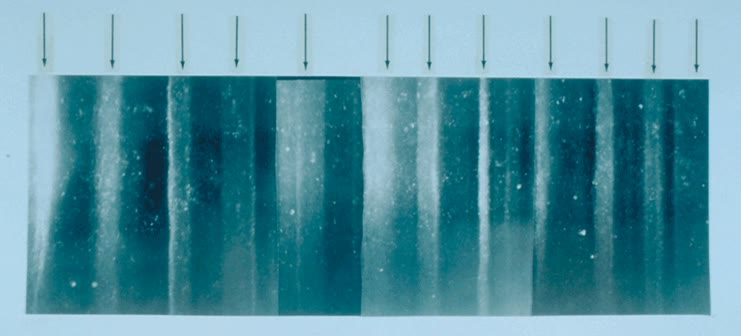
\includegraphics[width=0.72\linewidth]{images/book4/b2-24-gisp2-layers.jpg}
\par\smallskip{\small 取自格陵兰中部 GISP2 冰芯、深度 \qty{1855}{m} 处的一段，自下方打光，
可见夏季与冬季交替的层理（箭头为原幻灯片所标）。
北半球夏季干燥时，来自北极加拿大和格陵兰沿岸的尘埃
被风带到冰盖上。
（Anthony Gow，U.S.\ Army Corps of Engineers CRREL，NOAA Paleoclimatology 幻灯片集，公有领域，
经由维基共享资源。）}
\end{omfigure}
% ledger: photo:b2-24-gisp2, noaa:gisp2-layers

\begin{inthelab}[切割冰芯]
\begin{minipage}[t]{0.54\linewidth}\vspace{0pt}
在某国家冰芯设施中，冰芯装在管中保存，每管一米长的冰芯，
存放于 \qty{-36}{\celsius} 的档案冷冻室内；科学家则在 \qty{-24}{\celsius} 的检查室里工作。
新冰芯到达后，便形成一条冰芯处理流水线：科学家与工作人员
对每一段进行测量、编目和切割，通常每天 \num{30} 至 \qty{35}{m}，
因此一根 \qty{1000}{m} 长的冰芯需要六至八周。一位研究人员用
刨具将冰芯表面刨光，并测量其电导率，这是确定和定年各层的关键；另一位
则锯下那些将分析其中封存空气的二氧化碳和甲烷的样段；
随后样品被运往负责测量的实验室。在 EPICA Dome C，每个 $\delta$D
剖面样品为 \qty{55}{cm} 长的冰。
\end{minipage}\hfill
\begin{minipage}[t]{0.42\linewidth}\vspace{0pt}
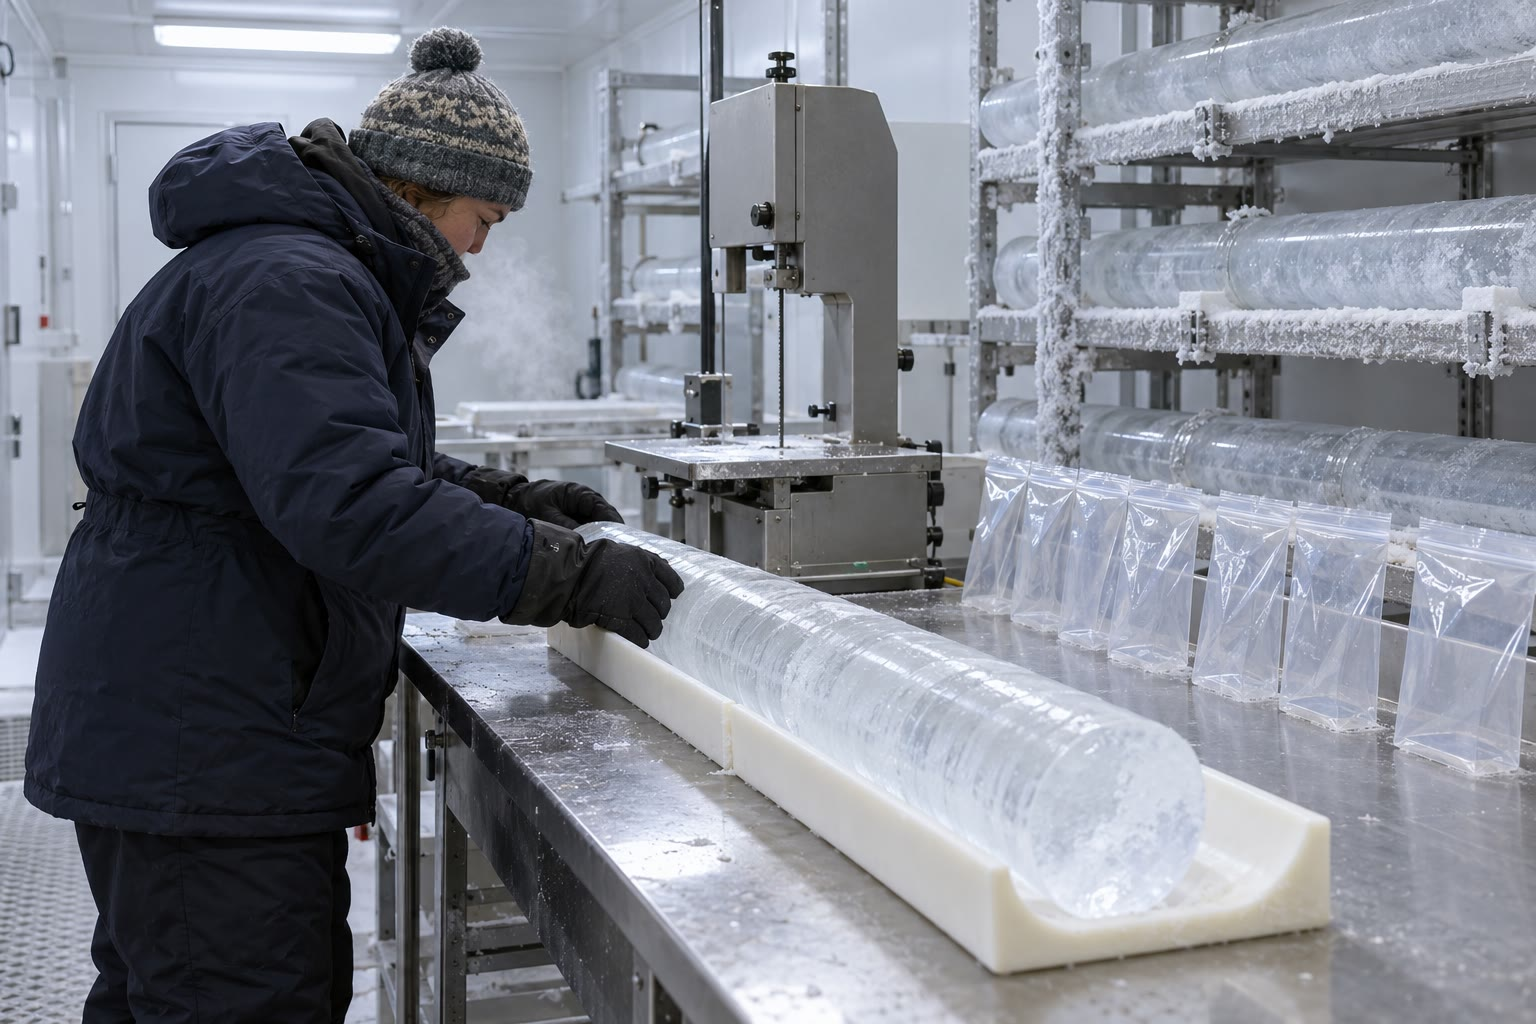
\includegraphics[width=\linewidth]{images/book4/ai/b2-24-cold-lab.jpg}

{\scriptsize 冷实验室工作台上的一段冰芯，旁边是带锯和样品
袋（AI 生成插图）。}
\end{minipage}
\end{inthelab}
% ledger: nsficf:cpl, jouzel07:edc-corr

\section{其他代用指标，其他档案}\label{sec:b2:climate-proxies:others}

\subsection*{贝壳中的镁}

有孔虫的方解石会以镁替代部分钙而摄入少量镁，
水温越高，摄入的镁越多。该比值不依赖于水的同位素组成，
因此它给出 $\delta^{18}$O 方程所需的温度。

\begin{definition}[Mg/Ca 比值（代用指标）]\label{def:b2:climate-proxies:mgca}
\emph{Mg/Ca 比值（代用指标）}\index{Mg/Ca 比值（代用指标）}是有孔虫壳体方解石中镁与钙的比值，
单位为 \unit{mmol/mol}，用作壳体生长时水温的度量，
由如下指数型标准曲线确定：
\[
  \text{Mg/Ca} = B\,\mathrm{e}^{A T},
\]
其中 $A$ 对浮游物种约为 \qty{0.09}{\per\celsius}，$B$ 因物种而异。
\end{definition}
% ledger: groeneveld19:anand, morley24:mgca, miller20:paleotemp

当 $A = 0.09$ 时，该比值每升高一度增长 $\mathrm{e}^{0.09} - 1 = \qty{9.4}{\percent}$，
与温度高低无关。对于一种生活在冷水中的浮游物种，仅由温度预测的标准曲线为
$\text{Mg/Ca} = 0.4\,\mathrm{e}^{0.09T}$；对 \num{235} 个壳体的拟合结果，壳体取自
浮游生物拖网和北大西洋岩芯顶部，结果为 $0.372\,\mathrm{e}^{0.0936T}$，其中 $r^2 = 0.90$。
在低温时，实测比值偏离该曲线，这一偏离被归因于
海水中碳酸根离子的浓度：代用指标很少只依赖单一变量。
底栖物种较不敏感，对于生活在沉积物中的低镁物种，
约每度 \qty{0.1}{mmol/mol}。
% ledger: morley24:mgca, wharton26:deep

\begin{omfigure}
\centering
% figdata/bachelor-2/proxies.py part calib
\begin{tikzpicture}
\begin{groupplot}[group style={group size=2 by 1, horizontal sep=1.7cm},
  tick label style={font=\scriptsize}, label style={font=\small}, height=5.2cm,
  width=0.48\linewidth]
\nextgroupplot[xmin=-2, xmax=14, ymin=0, ymax=3.8, xlabel={$T$ (\unit{\celsius})},
  ylabel={$\delta^{18}\mathrm{O}_{\mathrm{b}} - \delta^{18}\mathrm{O}_{\mathrm{sw}}$（千分值）},
  xtick={0,4,...,12}, title={a\enspace 底栖 $\delta^{18}$O}, title style={font=\scriptsize}]
\addplot[black, thick] table[x=T, y=dd_benthic] {figdata/out/bachelor-2-proxies-calib.dat};
\nextgroupplot[xmin=0, xmax=30, ymin=0, ymax=6.5, xlabel={$T$ (\unit{\celsius})},
  ylabel={Mg/Ca (\unit{mmol/mol})}, xtick={0,5,...,30}, title={b\enspace 浮游 Mg/Ca},
  title style={font=\scriptsize},
  legend style={font=\scriptsize, at={(0.03,0.97)}, anchor=north west, draw=none},
  legend cell align=left]
\addplot[ocRed, thick] table[x=T, y=mgca_pred] {figdata/out/bachelor-2-proxies-calib.dat};
\addlegendentry{$0.4\,\mathrm{e}^{0.09T}$}
\addplot[ocBlue, thick, densely dashed] table[x=T, y=mgca_fit]
  {figdata/out/bachelor-2-proxies-calib.dat};
\addlegendentry{$0.372\,\mathrm{e}^{0.0936T}$}
\end{groupplot}
\end{tikzpicture}
\par\smallskip{\small 两种标准曲线。（a）底栖标准曲线
（\cref{prop:b2:climate-proxies:benthic}）：方解石（按各自刻度）比水重，
每降温一度，重出 \num{0.21} 千分值。（b）一种浮游物种的 Mg/Ca，
分别由温度单独预测及拟合 \num{235} 个壳体所得。}
\end{omfigure}
% ledger: miller20:paleotemp, morley24:mgca

在同一批壳体上测得的 Mg/Ca 与 $\delta^{18}$O 给出关于两个未知量的两个方程：Mg/Ca
给出 $T$，再由\cref{prop:b2:climate-proxies:benthic}
得到 $\delta^{18}\mathrm{O}_{\mathrm{sw}}$，即冰量信号。将此方法应用于西北大西洋深部的底栖壳体，
该方法发现，末次盛冰期的海水仅比今天的冷约
\qty{2}{\celsius}（$-1.78 \pm \qty{0.56}{\celsius}$），而由孔隙水得到的估计
表明两个深层水团在冰期海洋中都接近冰点，分别为 $-1.1$ 和
\qty{-1.9}{\celsius}，而如今分别为 2 至 \qty{4}{\celsius} 与 0 至 \qty{1}{\celsius}。
% ledger: miller20:paleotemp, wharton26:deep

\subsection*{树轮}

\begin{definition}[树轮气候学；交叉定年]\label{def:b2:climate-proxies:dendro}
\emph{树轮气候学}\index{树轮气候学}是利用树木逐年形成的生长年轮重建过去气候的方法，
依据年轮的宽度、木材密度及其同位素组成进行重建。
\emph{交叉定年}\index{交叉定年}是比对不同树木之间宽窄年轮的排列格局，
从而为每一个年轮确定其绝对的日历年份，
并发现单棵树上局部缺失的年轮。
\end{definition}
% ledger: bebchuk26:crossdating, bebchuk26:absent-rings, ncei:tree-ring, ncei:proxy

年轮越宽，表明生长条件越有利。\omterm{def:b2:climate-proxies:dendro}{交叉定年}在气候极端的地点最为可靠，
那里有单一气候因子限制所有树木的生长，因而它们呈现相同的年轮格局；
在无单一因子占主导、且许多年轮局部缺失的地方，\omterm{def:b2:climate-proxies:dendro}{交叉定年}可能失效。
将现生树木、古木料与埋藏木材的年轮格局相互叠合，可将年表逐年向前延伸；
近期一项研究将英格兰东部 100 棵亚化石紫杉的年表定为
公元前 2668 至公元前 2213 年共 456 年，所用的是其中超过 \num{1500} 个年轮的 $\delta^{18}$O，
与经绝对定年的橡树年表比对。国际树轮数据库收存了年轮
宽度、密度、同位素及年表数据，涵盖六大洲超过 \num{5000} 个地点。
% ledger: ncei:proxy, bebchuk26:crossdating, bebchuk26:absent-rings, ncei:tree-ring

\subsection*{洞穴与湖泊}

\begin{definition}[洞穴沉积物；纹泥]\label{def:b2:climate-proxies:archives}
\emph{洞穴沉积物}\index{洞穴沉积物}是由地下水在洞穴内形成的矿物沉积体，
包括石笋、钟乳石及其他形态。\emph{纹泥}\index{纹泥}是
湖泊或海底沉积物中一年所形成的沉积层，通常由一对成分不同的纹层组成，
一层形成于夏季，另一层形成于一年中的其余时段。
\end{definition}
% ledger: ncei:speleothem, mccarthy23:varves

\omterm{def:b2:climate-proxies:archives}{洞穴沉积物}由渗入洞穴的地下水逐层生长；其层的厚度
及其同位素记录可反映过去的气候条件。有些具有逐年成层的纹带，
另有一些含有可用放射性方法定年的化合物。格陵兰冰芯的时间尺度与
葫芦洞\omterm{def:b2:climate-proxies:archives}{洞穴沉积物}的时间尺度在过去 \num{60000} 年内相差不超过 800 年：两种
用不同方法定年的档案相互印证。
% ledger: ncei:speleothem, svensson08:gicc05

\begin{omfigure}
\centering
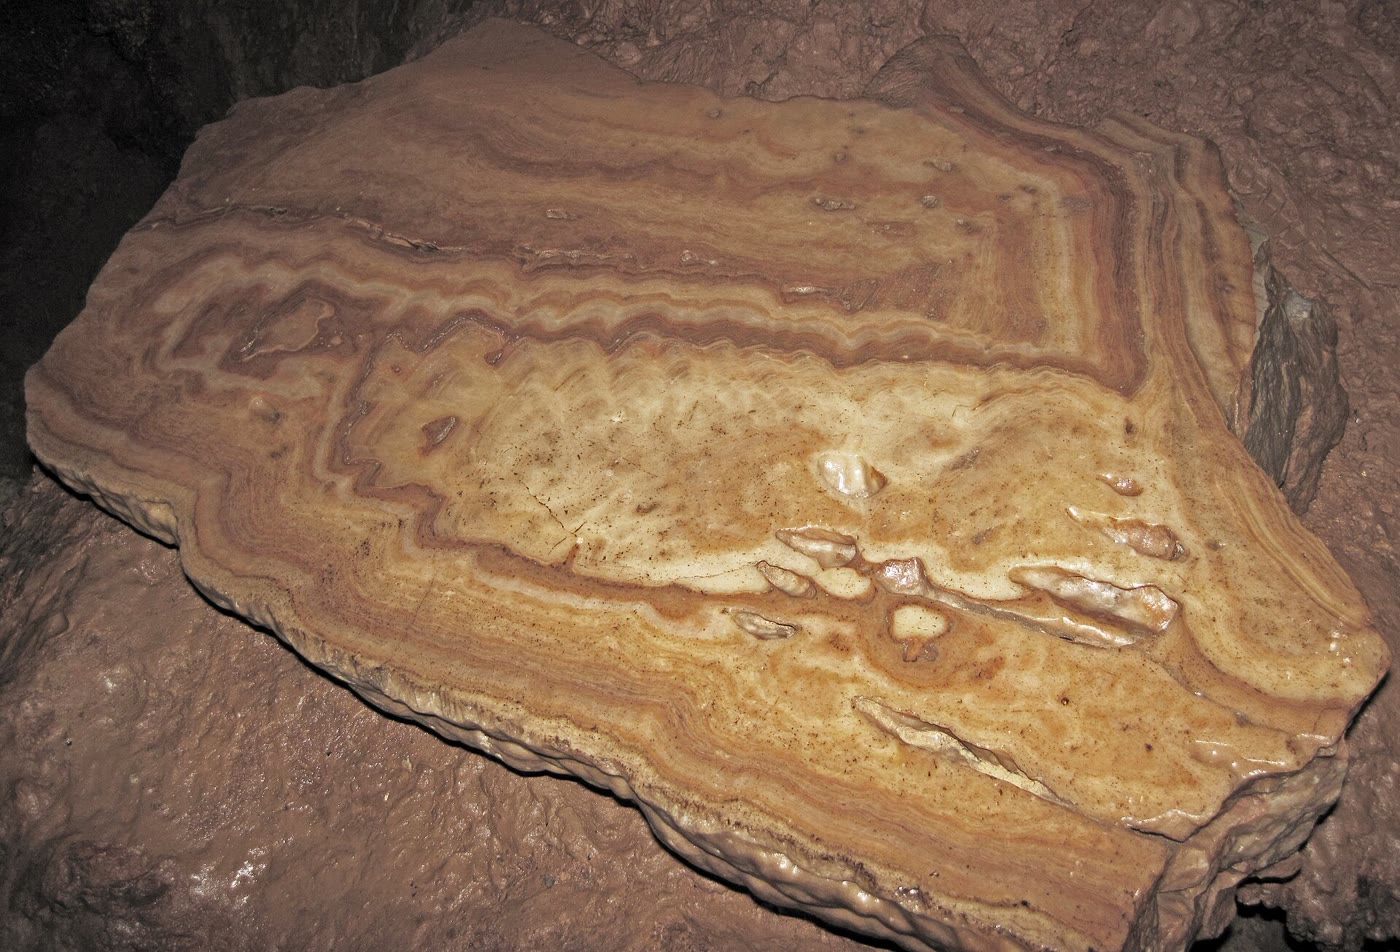
\includegraphics[width=0.62\linewidth]{images/book4/b2-24-speleothem.jpg}
\par\smallskip{\small 来自肯塔基州钻石洞穴的方解石\omterm{def:b2:climate-proxies:archives}{洞穴沉积物}切割抛光剖面，
因含氧化铁杂质而呈色：每一条带曾是沉积物的表面。
（James St.~John, CC BY 2.0，经维基共享资源。）}
\end{omfigure}
% ledger: photo:b2-24-speleothem

位于安大略省的克劳福德湖深盆中，湖底水体比上层水更咸、碱性更强，
其中没有能够搅动淤泥的较大动物，尽管水体含氧充足，
每年都会形成一个纹层对：先是一层有机质，
其上覆盖着每年夏季从碱性表层水中沉淀出的方解石。湖泊沉积物还保存了
周围植被的花粉，可用孢粉分析加以解读；无论是否具\omterm{def:b2:climate-proxies:archives}{纹泥}结构，它们都记录着
陆地的信息。
% ledger: mccarthy23:varves, mccarthy23:no-bioturbation, ncei:pollen

\section{年龄模型}\label{sec:b2:climate-proxies:age}

没有年代的代用指标只是一种奇闻。每一份档案都需要
建立深度（或年轮、层位）与年龄之间的关系。

\begin{definition}[年龄模型；年层计数]\label{def:b2:climate-proxies:age-model}
\emph{年龄模型}\index{年龄模型}是为档案中的每一个深度
赋予年龄及其不确定度的函数。\emph{年层计数}\index{年层计数}通过
自上而下数出每一层记录一年的层（冰层、\omterm{def:b2:climate-proxies:archives}{纹泥}、纹层）来构建年龄模型，
年代性质存疑的层计为
半年加减半年。
\end{definition}
% ledger: svensson08:gicc05, mccarthy23:varves

\begin{method}[建立年龄模型]\label{met:b2:climate-proxies:age-model}
\begin{enumerate}
  \item 若档案具有逐年层位，则自已知的顶部开始计数，
        将存疑的层单独记录。
  \item 若无逐年层位或无法分辨，则确定\emph{控制点}：
        经独立定年的深度，可用放射性碳或其他放射性方法定年、用已定年的火山灰定年，或与
        定年可靠的记录相匹配。
  \item 在控制点之间进行插值：若无更好的依据，则按深度线性插值，
        或依据档案的堆积与减薄过程建立模型。
  \item 将每一步的不确定度传递到每一个深度。
\end{enumerate}
\end{method}
% ledger: svensson08:gicc05, noaa:gisp2-layers, ncei:speleothem

格陵兰冰芯年代学 2005（GICC05）在三根格陵兰冰芯中计数逐年层，
其中冰期部分仅取自 NorthGRIP 冰芯，时段为过去 \num{60000} 年；其年龄
以公元 2000 年以前的年数表示，记作 b2k。存疑的层计为 $\frac12 \pm \frac12$，
累加得到\emph{最大计数误差}，作者将其视为两个标准差。
在全新世开始时，即 11\,703 年 b2k，其值为 50 年；在格陵兰间冰段 17 开始时，
即 \num{59440} 年 b2k，其值为 \num{1287} 年。
% ledger: svensson08:gicc05, svensson08:table1

\begin{proposition}[计数误差的增长]\label{prop:b2:climate-proxies:counting}
设一次计数包含 $n$ 个存疑层，每层计为 $\frac12$，其误差的标准差为
$\frac12$。若各层的误差相互独立，则总计数的标准差为
$\frac12\sqrt{n}$；若各层误差符号相同，则总计数的误差为
$\frac12 n$。
\end{proposition}

\begin{proof}
独立误差之和的方差等于各自方差之和：$n \times
(\frac12)^2$，其平方根为 $\frac12\sqrt{n}$。若各层误差方向相同，则
误差按数值相加：$n \times \frac12$。
\end{proof}

在 GI-17 处，\num{1287} 年的最大计数误差意味着 \num{2574} 个存疑层。若
各层误差相互独立，总计数的不确定度仅为 $\frac12\sqrt{2574} = 25$ 年。
线性相加是较为稳妥的选择：同一段冰层中的存疑层由同一批计数者
依据相同标准判定，没有理由认为它们的误差会相互抵消。
记录中较老的部分由两位作者独立计数，两人的计数结果
相差小于绝对误差，但在局部上超过了最终计数误差。
最大计数误差平均约为全新世某一段时间跨度的 \qty{1}{\percent}，
冰期部分为 \qty{5}{\percent}。
% ledger: svensson08:gicc05, svensson08:table1, svensson08:two-counters

\begin{omfigure}
\centering
% figdata/bachelor-2/proxies.py part gicc05
\begin{tikzpicture}
\begin{groupplot}[group style={group size=2 by 1, horizontal sep=1.7cm},
  tick label style={font=\scriptsize}, label style={font=\small}, height=5.4cm,
  width=0.48\linewidth, xmin=0, xmax=62, xlabel={GICC05 年龄（\unit{ka} b2k）}]
\nextgroupplot[ymin=1450, ymax=2450, y dir=reverse, ylabel={NorthGRIP 深度（\unit{m}）},
  title={a\enspace 深度与年龄}, title style={font=\scriptsize}]
\addplot[black, mark=*, mark size=1.1pt] table[x=age_ka, y=depth_m]
  {figdata/out/bachelor-2-proxies-gicc05.dat};
\nextgroupplot[ymode=log, ymin=2, ymax=30000, ylabel={不确定度（年）},
  title={b\enspace 计数不确定度}, title style={font=\scriptsize},
  legend style={font=\scriptsize, at={(0.03,0.97)}, anchor=north west, draw=none},
  legend cell align=left]
\addplot[ocRed, mark=*, mark size=1.1pt] table[x=age_ka, y=err_yr]
  {figdata/out/bachelor-2-proxies-gicc05.dat};
\addlegendentry{最大计数误差}
\addplot[ocBlue, mark=o, mark size=1.1pt] table[x=age_ka, y=err_random_yr]
  {figdata/out/bachelor-2-proxies-gicc05.dat};
\addlegendentry{若误差相互独立}
\end{groupplot}
\end{tikzpicture}
\par\smallskip{\small GICC05 年代学框架，覆盖从全新世开始至
\qty{59.44}{ka} 之间的 18 个气候事件：(a) NorthGRIP 岩芯的深度随年龄的变化，曲线趋于平缓，
原因是年层随深度变薄，每千年所占的冰层厚度减少；(b) 最大计数误差，以及同样数目的
存疑层若误差相互独立时给出的误差（\cref{prop:b2:climate-proxies:counting}）；
对数刻度。数据来源：Svensson et al.\ (2008)，表 1。}
\end{omfigure}
% ledger: svensson08:table1, svensson08:gicc05

年层随深度变薄，原因在于冰体下沉时发生流动并铺展：全新世开始至
GI-1 之间，NorthGRIP 的平均层厚为 \qty{3.75}{cm}；GI-16 至
GI-17 之间为 \qty{1.54}{cm}；在 \qty{100}{ka} 附近，流动模型给出约 \qty{1}{cm}。层越薄，
就越难将它们区分开来。
% ledger: svensson08:table1, svensson08:gicc05

\section{标定}\label{sec:b2:climate-proxies:calibration}

每一个从代用指标读出的数值，都要经过标定。

\begin{definition}[代用指标标定]\label{def:b2:climate-proxies:calibration}
称\emph{代用指标标定}\index{代用指标标定}为将代用指标的数值换算为其所代表的
气候变量的经验关系或理论关系，它建立在两者均已知的样本之上，
并附有其不确定度，以及其有效的
条件范围。
\end{definition}
% ledger: morley24:mgca, miller20:paleotemp

两者均已知的样本都是现代样本：浮游拖网中捕获的贝壳，沉积岩芯顶部与其上方海水的对比，近期降雪与其所在地
气温的对比，以及树木外围年轮与气象站记录的对比。
该关系随后用最小二乘法拟合；对于指数规律，如 Mg/Ca
标定，拟合在对数上进行，使 $\text{Mg/Ca} = B\,\mathrm{e}^{AT}$ 化为
直线 $\ln(\text{Mg/Ca}) = \ln B + AT$。标定须在未用于拟合的样本上加以验证：
将部分现代数据留出，用其进行预测。
% ledger: morley24:mgca, werner18:slopes, ncei:tree-ring

仍有三点限制。在空间上测得的标定，即今天不同地点之间的对比，未必能在时间上成立，
格陵兰冰芯已经表明了这一点。在今天的条件范围内测得的标定，
外推时须格外谨慎：贝壳的 Mg/Ca 在低温时偏离其规律，此时另一变量碳酸根离子起主导作用。
另外，在小范围内呈线性的关系，在大范围内未必仍是线性的，
\omterm{def:b2:climate-proxies:ice-volume}{冰量效应}便是如此。本章的方法以同一方式应对这些问题：
在同一样本上测量两种独立的代用指标，
让每一种指标检验另一种。
% ledger: werner18:slopes, morley24:mgca, rohling21:linear

\section*{练习}\label{sec:b2:climate-proxies:exercises}

除非另有说明，练习所用数据如下：平均海洋深度 $H = \qty{3682.2}{m}$，海洋
面积 \qty{361.84e6}{km^2}；底栖标定见\cref{prop:b2:climate-proxies:benthic}；
浮游标定为 $\text{Mg/Ca} = 0.4\,\mathrm{e}^{0.09T}$（\unit{mmol/mol}，\unit{\celsius}）；
$\delta$ 值：水体与冰以‰（\omterm{def:b2:isotope-geochemistry:standards}{VSMOW}）计，方解石以‰（\omterm{def:b2:isotope-geochemistry:standards}{VPDB}）计。
% ledger: charette:ocean-volume, miller20:paleotemp, morley24:mgca

\begin{exercise}[$\star$]\label{exo:b2:climate-proxies:1}
今天大陆冰盖约含 \qty{27.5e6}{km^3}，海洋约含 \qty{1350e6}{km^3}，
的水（将体积视为水的量）。(a) 若冰的平均 $\delta^{18}$O 为 $-30$‰，海洋为 0，
忽略淡水，求整个水圈的 $\delta^{18}$O。(b) 若所有冰全部融化，
海洋的 $\delta^{18}$O 将变为多少？(c) 水中
冰所占的比例是多少？
\end{exercise}
% ledger: white13c9:ice-mass

\begin{exercise}[$\star$]\label{exo:b2:climate-proxies:2}
某底栖贝壳的 $\delta^{18}\mathrm{O}_{\mathrm{b}} = 2.50$‰。(a) 若海水的 $\delta^{18}\mathrm{O}_{\mathrm{sw}} = 0$，
求其温度。(b) 若海水为 $+1.0$‰，求其温度。(c) 另一贝壳生活在 $0$‰ 的同一水体中，
其值为
$2.71$‰：该水体的温度低了多少？
\end{exercise}
% ledger: miller20:paleotemp

\begin{exercise}[$\star$]\label{exo:b2:climate-proxies:3}
(a) 求浮游标定在 \qty{10}{\celsius} 与 \qty{20}{\celsius} 时的 Mg/Ca 比值。
(b) 在这十度之间，该比值增大为原来的多少倍？平均每度增长百分之多少？
(c) 求 Mg/Ca 分别为 2.0 和
\qty{1.0}{mmol/mol} 的贝壳的温度。
\end{exercise}
% ledger: morley24:mgca

\begin{exercise}[$\star$]\label{exo:b2:climate-proxies:4}
某亚化石紫杉的年代序列跨越公元前 2668 年至公元前 2213 年。(a) 若两端年份均计算在内，
该序列共覆盖多少年？(b) 为什么由多棵树建立的年代序列比单棵树的年轮计数更值得信赖？
(c) 为什么你会预料，
对于靠近寒冷林线的树木，\omterm{def:b2:climate-proxies:dendro}{交叉定年}比温和湿润的低地森林中的树木更容易？
\end{exercise}
% ledger: bebchuk26:crossdating

\begin{exercise}[$\star\star$]\label{exo:b2:climate-proxies:5}
(a) 利用\cref{prop:b2:climate-proxies:mass-balance}，计算海平面下降 \qty{125}{m} 与
\qty{134}{m} 时的\omterm{def:b2:climate-proxies:ice-volume}{冰量效应}，冰取 $-40$‰。(b) 对
\qty{130}{m} 的下降，分别计算冰取 $-30$‰、$-35$‰ 和 $-50$‰ 时的\omterm{def:b2:climate-proxies:ice-volume}{冰量效应}。
(c) 冰的平均组成为何值时，\qty{130}{m} 的海平面下降所产生的效应恰好等于孔隙水中测得的 \num{1.0}‰？
并与现今冰盖的组成作比较。
\end{exercise}
% ledger: ipcc:lgm-sea, white:d18o, miller20:ice-cal, wharton26:deep

\begin{exercise}[$\star\star$]\label{exo:b2:climate-proxies:6}
比较同一浮游物种的 Mg/Ca 的两种校准：一种仅由温度给出的预测式，
即 $0.4\,\mathrm{e}^{0.09T}$，另一为拟合式 $0.372\,\mathrm{e}^{0.0936T}$。(a) 二者在何
温度下相等？(b) 在 \qty{2}{\celsius} 时，拟合比值比预测值低百分之几？
(c) 在 \qty{2}{\celsius} 下生长的壳体遵循拟合规律，
若按预测式计算，其温度应为多少？
\end{exercise}
% ledger: morley24:mgca

\begin{exercise}[$\star\star$]\label{exo:b2:climate-proxies:7}
在 NorthGRIP 岩芯中，全新世起点位于 \qty{1492.45}{m}，年龄为 \num{11703} 年 b2k，
GI-1 的起点位于 \qty{1604.64}{m}，年龄为 \num{14692} 年；GI-16 的起点位于
\qty{2402.55}{m}，年龄为 \num{58280} 年，GI-17 的起点位于 \qty{2420.44}{m}，年龄为 \num{59440} 年。
(a) 计算各区间内年层的平均厚度。(b) 为何深处的年层更薄，
(c) 为何在某一深度以下，\omterm{def:b2:climate-proxies:age-model}{年层计数}变得不可能？
\end{exercise}
% ledger: svensson08:table1, svensson08:gicc05

\begin{exercise}[$\star\star$]\label{exo:b2:climate-proxies:8}
取 \cref{exo:b2:climate-proxies:7} 中前两个控制点，其最大计数误差分别为 50
和 93 年。(a) 按深度作线性插值，求 \qty{1550}{m} 处冰的年龄。
(b) 以 1950 年以前的年数表示。(c) 以同样方法内插不确定度。
\end{exercise}
% ledger: svensson08:table1

\begin{exercise}[$\star\star$]\label{exo:b2:climate-proxies:9}
GICC05 的最大计数误差在 GI-1 处为 93 年，在 GI-17 处为 \num{1287} 年。(a) 每处各对应
多少个不确定的层？(b) 若这些层的误差相互独立，每层标准差为半年，则不确定度为多少？
(c) 线性和超出独立估计的倍数各为多少，
为何该倍数随深度增大？
\end{exercise}
% ledger: svensson08:gicc05, svensson08:table1

\begin{exercise}[$\star\star\star$]\label{exo:b2:climate-proxies:10}
在 EPICA Dome C，过去两千年冰的平均 $\delta$D 为 $-396.6$‰，
而在 19 至 \qty{23}{ka} 间为 $-441.7$‰。(a) 南极 $\delta^{18}$O 空间斜率为
\num{0.8}‰（每摄氏度）。借助\omterm{prop:b2:isotope-geochemistry:mwl}{大气降水线}，将其换算为 $\delta$D 的斜率，并
估算冰期降温。(b) 冰期海洋的 $\delta^{18}$O 偏重 \num{1.0}‰，
故由其形成的雪也偏重。若假设海洋的 $\delta$D 变化为其八倍，
则订正冰期的 $\delta$D，并重新估算降温。
(c) 已发表的两个时段温度距平分别为 $-0.09$ 和 \qty{-9.39}{\celsius}，由此隐含的
每摄氏度 $\delta$D 斜率为多少？已发表序列中还包含何种其他订正？
\end{exercise}
% ledger: data:b4-proxies, werner18:slopes, kc98:mwl, wharton26:deep, jouzel07:edc-corr

\begin{exercise}[$\star\star\star$]\label{exo:b2:climate-proxies:11}
某浮游物种 Mg/Ca 的校准采用了六个表层岩芯样品（水温，
Mg/Ca 单位为 \unit{mmol/mol}）：(4, 0.59), (8, 0.80), (12, 1.21), (16, 1.65), (20, 2.47), (24, 3.41)。
(a) 用最小二乘法拟合 $\ln(\text{Mg/Ca}) = \ln B + AT$，并给出 $A$ 与 $B$。(b) 计算
对数残差，并将拟合与规律 $0.4\,\mathrm{e}^{0.09T}$ 作比较。(c) 给出
Mg/Ca = 1.30 的冰期壳体的温度。(d) 某壳体 Mg/Ca = 0.45，计算其
温度，并说明为何该数值比前一个更不可信。
\end{exercise}
% ledger: morley24:mgca

\begin{exercise}[$\star\star\star$]\label{exo:b2:climate-proxies:12}
冰盖分两个阶段增长：首先，相当于 \qty{60}{m} 海平面变化的水以 $-30$‰ 的冰形式储存，
然后又以 $-45$‰ 的冰储存 \qty{70}{m}。(a) 证明：
\cref{prop:b2:climate-proxies:mass-balance}中的质量平衡化为 $(H - h)\,\Delta\delta = -\sum_i h_i\delta_i$，
对若干储冰库成立，并计算每一阶段后的\omterm{def:b2:climate-proxies:ice-volume}{冰量效应}。(b) 末态冰的平均
组成为何？(c) 一条依据末态校准的线性规则，可将
$\Delta\delta$ 换算为海平面变化。该规则对第一阶段推断的海平面下降是多少，
又为何会出错？
\end{exercise}
% ledger: rohling21:linear, white:d18o, miller20:ice-cal

\begin{problem}[{周末问题 --- 一个壳体，两种信号}]\label{pb:b2:climate-proxies:1}
末次盛冰期时深海低温了多少？底栖壳体的 $\delta^{18}$O 与冰量混杂在一起，
本题将二者分开。利用习题中的数据，
海平面比今天低 125 至 \qty{134}{m}，据认为北美冰盖的冰
$\delta^{18}$O 约为 $-40$‰。

\medskip\noindent\textbf{第一部分 --- 陆地上的冰。}
\begin{enumerate}
  \item 计算海平面下降 \qty{130}{m} 时从海洋中移走的水的体积。
  \item 取冰为 $-40$‰，计算该下降所对应的\omterm{def:b2:climate-proxies:ice-volume}{冰量效应}。
  \item 计算下降 \qty{125}{m} 与 \qty{134}{m} 时的\omterm{def:b2:climate-proxies:ice-volume}{冰量效应}。
  \item 对 \qty{130}{m} 的下降，分别取冰为 $-35$‰ 与 $-50$‰，计算\omterm{def:b2:climate-proxies:ice-volume}{冰量效应}。哪一项
        不确定度影响更大，是海平面的还是冰的？
  \item 冰期沉积物孔隙水给出 $1.0 \pm 0.1$‰，要产生这一数值，
        需要下降 \qty{130}{m} 时冰的平均组成为多少？
  \item 取冰为 $-40$‰，计算小幅海平面下降时的每米偏移量，并
        与由定年海平面推得的每米 \num{0.011}‰ 数值作比较。
\end{enumerate}

\medskip\noindent\textbf{第二部分 --- 两支温度计。}
\begin{enumerate}[resume]
  \item 由\cref{prop:b2:climate-proxies:benthic}可知，水体成分不变时，降温 \qty{1}{\celsius} 使
        $\delta^{18}\mathrm{O}_{\mathrm{b}}$ 升高 \num{0.21}‰。
  \item 计算今日生长的底栖壳体的 $\delta^{18}\mathrm{O}_{\mathrm{b}}$，其水温为
        \qty{2.0}{\celsius}，水的 $\delta^{18}\mathrm{O}_{\mathrm{sw}} = 0$。
  \item 计算冰期壳体的值，其生长水温为 \qty{-1.0}{\celsius}，
        水的 $\delta^{18}\mathrm{O}_{\mathrm{sw}} = +1.0$‰。两壳体之间的变化为多少，
        其中有多少来自水体成分？
  \item 某浮游壳体的 Mg/Ca = \qty{2.0}{mmol/mol}，计算其温度。
  \item 低镁底栖壳体每度约增加 \qty{0.1}{mmol/mol}。某冰期壳体的
        Mg/Ca 比同一地点、同一物种的现代壳体低 \qty{0.18}{mmol/mol}，
        这意味着降温多少？
  \item 为何 Mg/Ca 给出的温度与冰量无关？
\end{enumerate}

\medskip\noindent\textbf{第三部分 --- 残差。}
LR04 叠加曲线今日读数为 \num{3.23}‰，19 至
\qty{23}{ka} 间平均值为 \num{4.92}‰。
\begin{enumerate}[resume]
  \item 计算叠加曲线从今日到末次盛冰期的变化量。
  \item 若其全部为\omterm{def:b2:climate-proxies:ice-volume}{冰量效应}，取冰为 $-40$‰，则将意味着
        多大的海平面下降（反解\cref{prop:b2:climate-proxies:mass-balance}）？这与
        海平面证据是否一致？
  \item 取第 2 题中的\omterm{def:b2:climate-proxies:ice-volume}{冰量效应}，则温度所剩残差为多少，
        由此得出深层水的降温为多少？
  \item 改取孔隙水的数值 \num{1.0}‰，则残差与降温各为多少？
  \item 另一重建采用每摄氏度 \num{0.25}‰ 的斜率，以此重复上述两项估算。
  \item 今日北大西洋深层水温为 2 至 \qty{4}{\celsius}，南极底层水为
        0 至 \qty{1}{\celsius}；孔隙水给出二者在冰期海洋中分别为 $-1.1$ 和 \qty{-1.9}{\celsius}，
        而底栖壳体的 Mg/Ca 显示西北大西洋深层仅冷约
        \qty{1.8}{\celsius}。这些结果给出的降温范围为多少，
        并且它们更支持第 15 题与第 16 题两种估计中的哪一种？
\end{enumerate}

\medskip\noindent\textbf{第四部分 --- 冰芯所见。}
在 EPICA Dome C，过去两千年的平均 $\delta$D 为 $-396.6$‰，并
在 19 至 \qty{23}{ka} 间为 $-441.7$‰；已发表的温度距平分别为 $-0.09$ 与
\qty{-9.39}{\celsius}。
\begin{enumerate}[resume]
  \item 计算 $\delta$D 的变化量。
  \item 取 $\delta^{18}$O 斜率为每摄氏度 \num{0.8}‰，并借助\omterm{prop:b2:isotope-geochemistry:mwl}{大气降水线}，
        估算 Dome C 处的降温。
  \item 计算已发表的降温，以及由此隐含的每摄氏度 $\delta$D 斜率。
  \item 末次盛冰期时全球平均地表温度低 5 至 \qty{7}{\celsius}。
        请将 Dome C、全球及深海的降温按大小排序。
  \item 为何深海的降温不可能与南极地表一样大？
  \item 综合来看：经孔隙水的\omterm{def:b2:climate-proxies:ice-volume}{冰量效应}订正后，末次盛冰期的深海
        比今日低温了多少？
\end{enumerate}
\end{problem}
% ledger: charette:ocean-volume, ipcc:lgm-sea, miller20:ice-cal, white:d18o, white13c9:ice-volume, wharton26:deep, miller20:paleotemp, morley24:mgca, data:b4-proxies, rohling21:linear, werner18:slopes, kc98:mwl, ipcc:lgm-cooling
